
\documentclass[a4paper,11pt]{article}

%% PREAMBLE %%

% Packages
\usepackage[utf8]{inputenc} % UTF-8 is a good thing I guess
\setcounter{secnumdepth}{0}
\usepackage[a4paper, total={150mm, 225mm}]{geometry} % use reasonable amount of the page
\usepackage{amsmath}  % allows unnumbered equations
\usepackage{textcomp} % explicitly imported to calm gensymb
\usepackage{gensymb}  % gives degree sign
\usepackage{tikz}     % allows drawing pretty diagrams
\usepackage{pgfplots} % allows graphs and plots
\usepackage{graphicx} % allows images
\usepackage{pdfpages} % allows to import other PDF pages
\usepackage{float}

%Prettifying packages
\usepackage[document]{ragged2e}
\usepackage[margin=1cm]{caption} % spacing for captions, 1cm in from border
\usepackage{subcaption} 
\usepackage{fancyhdr}
\pagestyle{fancy}
\usepackage[normalem]{ulem}
\usepackage{colortbl}
\usepackage{xcolor}
\usepackage{listings}

%make numbers not selectable
\usepackage{accsupp}
\renewcommand{\thelstnumber}{% Line number printing mechanism
  \protect\BeginAccSupp{ActualText={}}\arabic{lstnumber}\protect\EndAccSupp{}
}
\usepackage[T1]{fontenc}
\usepackage[framed,numbered]{matlab-prettifier} %print pretty code
\usepackage{epstopdf}


% Titlepage variables
%\title{SA1: Final Report}
%\author{Paul Wernicke (pw444)\\Group 4}
%\date{May 2020}

\lhead{Week 1 Report}
\rhead{Jonathan Collins \& Paul Wernicke}
\lfoot{jc2071 \& pw444}

%% DOCUMENT %%
\pagenumbering{gobble}
\begin{document}
%\maketitle
\begin{titlepage}
    \begin{center}
 
        \LARGE
        SA1: Aircraft Wing Analysis
        
        \vspace{0.1cm}
        
        \LARGE
        
        Interim Report 1
        
        \vspace{0.4cm}
        
        \large
        
        Jonathan Collins \& Paul Wernicke
        
        \vspace{0cm}
        
        Homerton College
        
        \vspace{0.3cm}
        
        Easter Term 2020
        
        \vspace{0.5cm}
        
        %\large
        
        %\textbf{Abstract}
        
        %\justify
        
        %\normalsize
        %I don't think we really need an abstract.
        %\tableofcontents
        \lstlistoflistings
        \listoffigures
    \end{center}
\end{titlepage}
\pagenumbering{arabic}

\section{Introduction}

\section{Changes to the code}
% here mention how we changed the lift drag ration in order to address somoe issures
%\begin{figure}[h]
\centering
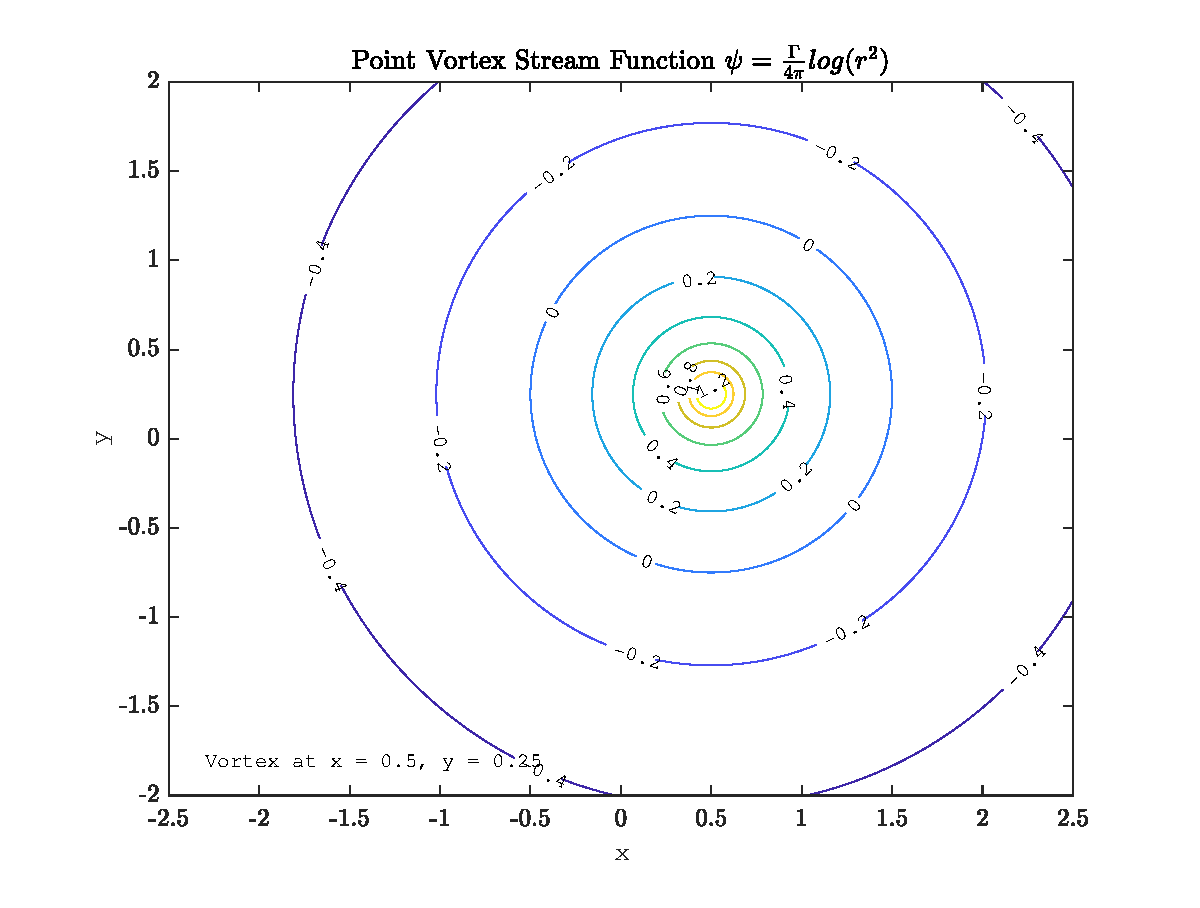
\includegraphics[scale=0.8]{untitled.eps}
\caption{Exercise 1.}
\label{foobar-figure}
\end{figure}


\end{document}